\documentclass{urdpl}     % praca w języku polskim

% Lista wszystkich języków stanowiących języki pozycji bibliograficznych użytych w pracy.
% (Zgodnie z zasadami tworzenia bibliografii każda pozycja powinna zostać utworzona zgodnie z zasadami języka, w którym dana publikacja została napisana.)
\usepackage[english,polish]{babel}

% Użyj polskiego łamania wyrazów (zamiast domyślnego angielskiego).
\usepackage{polski}

\usepackage[utf8]{inputenc}

% dodatkowe pakiety

\usepackage{mathtools}
\usepackage{amsfonts}
\usepackage{amsmath}
\usepackage{amsthm}
\usepackage[hidelinks]{hyperref}
\usepackage{float}
\usepackage{listings}
\usepackage{graphicx}
\usepackage{subcaption}
\usepackage{booktabs} % Dla \toprule, \midrule, \bottomrule
\usepackage{multirow} 
\usepackage{tabularx} 
\usepackage{amssymb} 
\usepackage{listings}
\usepackage{xcolor}
\usepackage{array}
\usepackage{makecell}
\usepackage[flushleft]{threeparttable}
\usepackage[normalem]{ulem}
\usepackage{lineno}
% ---------------------------------------------

% --- < bibliografia > ---

\usepackage{csquotes}

% ------------------------
% --- < listingi > ---

% Użyj czcionki kroju Courier.
\usepackage{courier}

\usepackage{listings}
\lstloadlanguages{TeX}
\renewcommand{\lstlistlistingname}{Spis listingów}
\renewcommand{\lstlistingname}{Listing}


\lstset{
	literate={ą}{{\k{a}}}1
           {ć}{{\'c}}1
           {ę}{{\k{e}}}1
           {ó}{{\'o}}1
           {ń}{{\'n}}1
           {ł}{{\l{}}}1
           {ś}{{\'s}}1
           {ź}{{\'z}}1
           {ż}{{\.z}}1
           {Ą}{{\k{A}}}1
           {Ć}{{\'C}}1
           {Ę}{{\k{E}}}1
           {Ó}{{\'O}}1
           {Ń}{{\'N}}1
           {Ł}{{\L{}}}1
           {Ś}{{\'S}}1
           {Ź}{{\'Z}}1
           {Ż}{{\.Z}}1,
	basicstyle=\footnotesize\ttfamily,
}

% defninicja stylu python
\lstdefinestyle{stylePython}{
    language=Python,
    commentstyle=\color{green},          % Kolor komentarzy
    keywordstyle=\color{blue},           % Kolor słów kluczowych
    numberstyle=\tiny\color{gray},       % Kolor i styl numerów linii
    stringstyle=\color{red},             % Kolor ciągów znaków
    basicstyle=\ttfamily\footnotesize,   % Podstawowy styl kodu
    breakatwhitespace=false,             % Automatyczne dzielenie wierszy
    breaklines=true,                     % Dzielenie długich linii
    keepspaces=true,                     % Zachowanie spacji
    numbers=left,                        % Numery linii po lewej
    numbersep=5pt,                       % Odstęp numerów od kodu
    showspaces=false,                    % Nie pokazuj spacji
    showstringspaces=false,              % Nie pokazuj spacji w ciągach znaków
    showtabs=false,                      % Nie pokazuj tabulacji
    tabsize=2                            % Rozmiar tabulacji
}

% defnicja stylu JAVA
\lstdefinestyle{javaStyle}{
    language=Java,
    basicstyle=\ttfamily\footnotesize,
    keywordstyle=\color{blue},
    commentstyle=\color{green!50!black}\itshape,
    stringstyle=\color{green},
    numberstyle=\tiny\color{gray},
    numbers=left,
    numbersep=5pt,                       % Odstęp numerów od kodu
    stepnumber=1,
    showspaces=false,                    % Nie pokazuj spacji
    tabsize=2,
    showstringspaces=false,
    breaklines=true,
    breakatwhitespace=false,             % Automatyczne dzielenie wierszy
    showtabs=false,                      % Nie pokazuj tabulacji
    keepspaces=true                    % Zachowanie spacji
}


\definecolor{stringcolor}{RGB}{163,21,21}    % pomarańczowy - stringi
\definecolor{typecolor}{RGB}{43, 145, 176}     % ciemny fiolet - klasy, typy

\lstdefinestyle{csStyle}{
    language=[Sharp]C, % dla C#; można zmienić na Java
    basicstyle=\ttfamily\footnotesize,
    keywordstyle=\color{blue},
    stringstyle=\color{stringcolor},
    commentstyle=\color{green!50!black}\itshape,
    morekeywords={class, public, private, protected, static, void, string, int, new}, % dodatkowe słowa kluczowe
    emphstyle=\color{typecolor}\bfseries, % klasy na fioletowo
    numbers=left,
    numbersep=5pt,                       % Odstęp numerów od kodu
    numberstyle=\tiny\color{gray},
    stepnumber=1,
    breaklines=true,
    showspaces=false,                    % Nie pokazuj spacji
    tabsize=2,
    showstringspaces=false,
    breakatwhitespace=false,             % Automatyczne dzielenie wierszy
    showtabs=false,                      % Nie pokazuj tabulacji
    keepspaces=true                    % Zachowanie spacji  
}

\definecolor{lightgray}{rgb}{0.9,0.9,0.9}
    % \definecolor{blue}{rgb}{0,0,1}
    \definecolor{green}{rgb}{0,0.6,0}
    % \definecolor{red}{rgb}{0.6,0,0}
    \definecolor{gray}{rgb}{0.5,0.5,0.5}

% % ------------------------
\AtBeginDocument{
	\renewcommand{\tablename}{Tabela}
	\renewcommand{\figurename}{Rys.}   
    \newcommand{\listingname}{Listing}
}


% ------------------------
% --- < tabele > ---

% defines the X column to use m (\parbox[c]) instead of p (parbox[t])
\newcolumntype{C}[1]{>{\hsize=#1\hsize\centering\arraybackslash}X}

%---------------------------------------------------------------------------

\author{Bartosz Buczuliński}
\shortauthor{B. Buczuliński}
\noAlbum{134894}

\titlePL{Symulator sklepu internetowego}
\titleEN{Online shop simulator}

\shorttitlePL{Symulator sklepu internetowego} % skrócona wersja tytułu jeśli jest bardzo długi
\shorttitleEN{Online shop simulator}

\thesistype{Praca projektowa}


\thesisDone{Praca wykonana pod kierunkiem}
\supervisor{mgr inż. Dawid Kosior}
%\supervisor{Jan Nowak PhD}

\degreeprogramme{Informatyka}
%\degreeprogramme{Computer Science}

\date{2025}

\department{Instytut Informatyki}
%\department{Institute of Computer Science}

\faculty{Wydział Nauk Ścisłych i Technicznych}
%\faculty{Faculty of Science and Technology}



\setlength{\cftsecnumwidth}{10mm}

%---------------------------------------------------------------------------
\setcounter{secnumdepth}{4}
\brokenpenalty=10000\relax

% --------------------------------------------------------------------------
% główna część pracy
% --------------------------------------------------------------------------

\begin{document}

\titlepages

% Ponowne zdefiniowanie stylu plain, aby usunąć numer strony z pierwszej strony spisu treści i poszczególnych rozdziałów.
\fancypagestyle{plain}
{
    % Usuń nagłówek i stopkę
    \fancyhf{}
    % Usuń linie.
    \renewcommand{\headrulewidth}{0pt}
    \renewcommand{\footrulewidth}{0pt}
}

\setcounter{tocdepth}{2}
\tableofcontents
\clearpage


% dodanie poszczególnych rozdziałów 

\chapter{Streszczenie w języku polskim i angielskim}
\label{cha:Streszczenie}

\section{Streszczenie w języku polskim.}

Projekt pt. "Symulator sklepu internetowego" ma na celu stworzenie aplikacji imitującej działanie realnego sklepu internetowego specjalizującego 
się w sprzedaży książek w różnych formatach: fizycznych, ebooków i audiobooków. Aplikacja została napisana w języku Java z wykorzystaniem technologii 
takich jak Swing dla interfejsu graficznego oraz MySQL dla zarządzania bazą danych. Głównym celem projektu było odzwierciedlenie pełnego procesu obsługi 
klienta, od rejestracji i logowania, przez przeglądanie oferty i składanie zamówień, po zarządzanie produktami i użytkownikami przez administratora. 
Aplikacja uwzględnia również rolę gościa, który może przeglądać ofertę bez konieczności logowania. Projekt spełnia wymagania funkcjonalne i niefunkcjonalne, 
takie jak wydajność, niezawodność i intuicyjność interfejsu.

\section{Streszczenie w języku angielskim.}

The project titled "Online Store Simulator" aims to create an application that mimics the operation of a real online store specializing in 
the sale of books in various formats: physical books, ebooks, and audiobooks. The application was developed in Java using technologies such as
 Swing for the graphical interface and MySQL for database management. The main goal of the project was to reflect the complete customer service process, 
 from registration and login, through browsing the offer and placing orders, to product and user management by the administrator. The application also includes a
  guest role, allowing users to browse the offer without logging in. The project meets functional and non-functional requirements, such as performance, reliability,
   and interface intuitiveness.
\chapter{Opis założeń projektu}
\label{cha:założenia}

\section{Założenia projektu}
\label{sec:zalozenia}

Projekt to symulator sklepu internetowego "BookHaven" specjalizującego się w sprzedaży książek w różnych formatach: książek fizycznych, ebooków oraz audiobooków.
Głównym celem aplikacji jest odzwierciedlenie pełnego, realnego procesu korzystania ze sklepu internetowego, od rejestracji i logowania, po przeglądanie
oferty i składanie zamówień po stronie klienta, a także możliwość zarządzania produktami, zamówieniami i użytkownikami po stronie administratora.



% ------------------------
\section{Wymaganie funkcjonalne}
\label{sec:wymagania funkconajle}


Zarządanie użytkownikami musi obejmować rejestrację nowych użytkowników oraz logowanie na konto. 
Każdy użytkownik ma przypisaną rolę, która określa jakie działania będzie mógł on podejmować w aplikacji.
Administrator ma mieć możliwość usuwania istniejących użytkowników oraz dodawania nowych administratorów,
natomiast po stronie klienta dostępna jest opcja aktualizacji danych potrzebnych do wysyłki. 

Klient może przeglądać całą ofertę, ma dostęp do filtrowania oraz sortowania produktów w ofercie oraz dodawania ich do koszyka,
w którym można przeglądać wybrane produkty, usunąć je z niego, oraz złożyć zamówienie.

Administrator ma mieć narzędzia pozwalające na zarządzanie produktami: dodawanie, edycja i usuwanie.

Proste zarządanie zamówieniami również musi odbywać się po stronie administratora. Dostępne ma być przeglądanie wszystkich zamówień, gdzie widnieją
dane zamawiającego oraz produkty które zamówił, dodatkowo, bezpośrednio w aplikacji, administrator ma możliwość zmiany statusu zamówienia.

Aplikacja obsługuje możliwość zalogowania się jako gość, gdzie nie ma potrzeby logowania, natomiast ma on
mieć wówczas dostęp jedynie do przeglądania oferty.


%---------------------------------------------------------------------------

\section{Wymaganie niefunkcjonalne}
\label{sec:wymagania niefunkcjonalne}

Istotna jest wydajność aplikacji, krótki czas ładowania poszczególnych stron aplikacji, a także bezproblemowa obsługa
rozbudowanej bazy produktów i użytkowników.

Niezawodność projektu powinna być zapewniona przez obsługę wyjątków dla, możliwie wszystkich, funkcjonalości aplikacji oraz 
informowanie użytkownika o jego błędnych działaniach.

Graficzny interfejs użytkownika musi być prosty i intuicyjy. Poszczególne panele aplikacji powinny być przejyżste, tak aby
klienci, goście i administratorzy nie mieli problemu z nawigowaniem po nich. Oprócz tego interfejst graficzny ma wyglądać estetycznie, każda strona 
aplikacji nie powinna odbiegać wizualnie od pozostałych dzięki zostosowaniu wszędzie jednolitego białego tła oraz banera w kolorze \texttt{BA2F33} z nazwą sklepu.

Możliwa ma być również skalowalność aplikacji, obejmująca zwiększającą się bazę produktów, użytkowników i zamówień, a także możliwość późniejszej
rozbudowy systemu o dodatkowe funkcjonalność, między innymi dodanie nowych metod płatności lub implementacja przechowywania produktów z koszyka w bazie.
\chapter{Opis struktury projektu}
\label{cha:struktura}

% ------------------------------------------------------------------------

\section{Struktura kodu projektu}

Projekt symulatora sklepu interentowego napisany został w języku obiektowym Java, zatem do jego uruchomienia niezbędne będzie oprogramwanie Java w wersji 11+. 
Projekt podzielony został na sześć pakietów:
\begin{itemize}
    \item	userPCG,
    \item	productPCG,
    \item	orderPCG,
    \item   shoppingCartPCG,
    \item   GUI,
    \item   figures,
    \item   database.
\end{itemize}

% ------------------------------------------------------------------------

\subsection{Użytkownicy}

Zarządanie użytkownikami, klasy i metody im poświęcone znajdują się w pakiecie \texttt{userPCG}. Klasa \texttt{User} zawiera pola informujące o danych użytkownika,
konstruktory oraz podstawowe metody, takie jak gettery i settery. Wewnątrz klasy \texttt{userServices} znajdują się kluczowe metody do zarządania użytkownikami w panelach klienta, jak i administratora, takie 
jak np. metoda do rejestrowania nowego użytkownika, przedstawiona na \listingname~\ref{registerUser}.

\lstinputlisting[caption= Metoda do rejestrowania nowych użytkowników, label=registerUser, style = javaStyle]{src/registerUser.java}

Natomiast zarządaniem aktualnie zalogowanym użytkownikiem zajmuje się klasa \texttt{UserSession}.
Każdy typ użytkownika ma przypisaną rolę, której odpowiada warość liczbowa, co zaprezentowane jest w \tablename~\ref{tabRole}.

\begin{table}[H]
    \caption{Role użytkowników}
    \label{tabRole}
    \centering
    \begin{tabular}{ccc}
        \toprule
        \textbf{rola} & \textbf{wartość liczbowa} \\ \toprule
        klient           & 1                              \\
        administrator           & 2                               \\
        gość           & 3                              \\
    \bottomrule
    \end{tabular}
\end{table}

Poszczególne typy użytkowników mają dostęp do różnych działań w aplikacji.

% ------------------------------------------------------------------------

\subsection{Produkty}

Wszystkie potrzebne informacje i metody do zarządzania produktami w sklepie zawarte są w pakiecie \texttt{productPCG}.
Każdy typ sprzedawanego produktu, czyli książki fizyczne, ebooki i audiobooki posiadają własne klasy (\texttt{PhysicalBook}, \texttt{Ebook}, \texttt{Audiobook}), które dziedziczą
po klasie abstrakcyjnej \texttt{Book}, która to z kolei implementuje interfejs \texttt{Product}, co przedstawia \figurename~\ref{fig2}. Diagram został sporządzony na stronie: \url{https://www.drawio.com/}.

\begin{figure}[H]
    \centering
    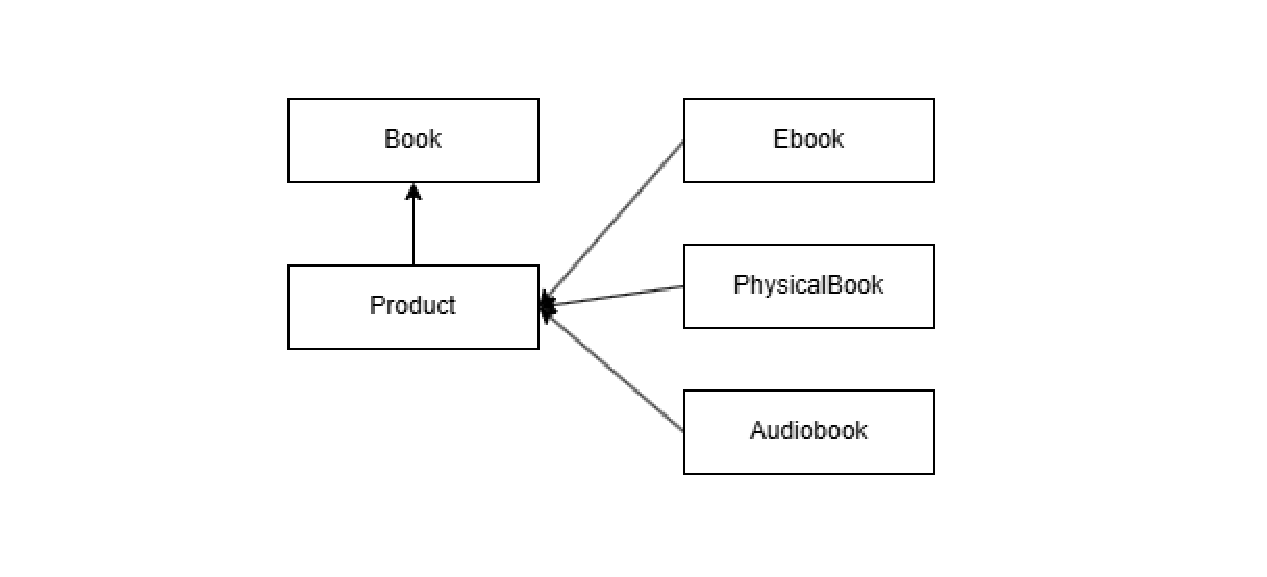
\includegraphics[width=\linewidth]{figures/fig_0002.eps}\\
    \caption{Diagram dziedziczenia klas produktów.\label{fig2}}
\end{figure}

Pakiet zawiera również enum \texttt{BookCategory}, w którym przechowywane są kategorie sprzedawanych książek. 
Enum przedstawiono na \listingname~\ref{enum}.
\lstinputlisting[caption= Enum kategorii książek, label=enum, style = javaStyle]{src/enum.java}

Kluczowe metody do zarządzania produktami znajdują się w klasie \texttt{ProductServices}.
Zawiera między innymi metody do dodawania, usuwania, pobierania, a także metody aktualizowania danych podstawowych produktu (\texttt{Book}) oraz pochodne 
metody do aktualizowania danych specyficznych dla konkretnych typów produktów (\texttt{PhysicalBook}, \texttt{Ebook}, \texttt{Audiobook}), których przykłady 
podano w \listingname~\ref{updateBook} i \listingname~\ref{updateEbook}.
\lstinputlisting[caption= Metoda aktualizująca podstawowe dane produktu, label=updateBook, style = javaStyle]{src/updateBook.java}
\lstinputlisting[caption= Metoda aktualizująca specyficzne dane dla Ebooka, label=updateEbook, style = javaStyle]{src/updateEbook.java}

Rozbudowany unikalny identyfikator produktu jest generowany automatycznie dzięki użyciu metody \texttt{randomUUID()} ze standardowej klasy \texttt{UUID}.

Wewnątrz klasy \texttt{ProductServices} umieszona została dodatkowo klasa wewnętrzna \texttt{ProductInfo}, która zawiera konkretne pola ułatwiające przechowywanie
informacji o produktach, np. w katalogach i koszyku. Zaprezentowana została ona w \listingname~\ref{productInfo}.
\lstinputlisting[caption= Wewnętrzna klasa ProductInfo, label=productInfo, style = javaStyle]{src/ProductInfo.java}

% ------------------------------------------------------------------------

\subsection{Koszyk i Zamówienia}

Obsługa zamówień odbywa się przy pomocy klasy \texttt{OrderServices} w pakiecie \texttt{orderPCG}. Oprócz metody do tworzenia nowego zamówienia i aktualizacji statusu zamówienia, dostępne są również metody 
tworzące listy wszystkich zamówień wykorzystujące wewnętrzne klasy \texttt{OrderInfo}, z polami dotyczącymi danych samego zamówinienia, a także \texttt{OrderItemInfo}, z polami produktów w zamówieniu.

Koszyk z produktami działający przy pomocy klasy \texttt{ShoppingCart} zawiera listę produktów, która później trafia do zamówienia, a także metody do dodawania dodawania i usuwania produktów z niego.

% ------------------------------------------------------------------------

\subsection{Materiały}

Jedynym zewnętrznym materiałem wykorzystywanym w aplikacji jest \texttt{book.png}, przechowywany w \texttt{figures}, materiał ten służy jako logo, wyświetlane w banerze na każdej stronie sklepu.
Logo to, przedstawione na  \figurename~\ref{fig3}, pobrane zostało z \url{https://icons8.com/icons/set/book}.
\begin{figure}[H]
    \centering
    
\includegraphics[width=\linewidth]{figures/fig_0003.eps}\\
    \caption{obrazek książki wykorzystany w aplikacji.\label{fig3}}
\end{figure}

% ------------------------------------------------------------------------

\section{Baza danych}

% ------------------------------------------------------------------------

W symulatorze sklepu internetowego, dane przechowywane i zarządzane są za pomocą relacyjnej bazy danych MySQL.

\subsection{Połączenie z bazą danych}

Połączenie z bazą danych odbywa się za pomocą interfejsu API, JDBC. Baza danych testowo przechowywana jest na serwerze pakietu XAMPP, natomiast połącznie z serwerem przeprowadzone zostało poprzez
implementację do projektu \texttt{Connector/J}, dostępnego na \url{https://dev.mysql.com/downloads/connector/j/}.

Celem łatwego łączenia się z bazą danych utworzona została klasa \texttt{DBConnection}, przedstawiona w \listingname~\ref{database}.
\lstinputlisting[caption= Klasa łączenia się z bazą danych, label=database, style = javaStyle]{src/database.java}

% ------------------------------------------------------------------------

\subsection{Struktura bazy danych}

Struktura bazy, zaprojektowana została w taki sposób, aby umożliwić łatwe zarządzanie informacjami o użytkownikach, produktach oraz zamówieniach.
Baza danych składa się z tabel głównych \texttt{users}, \texttt{products} i \texttt{orders}, a także tabel \texttt{physical book}, \texttt{ebooks}, \texttt{audiobooks} z danymi specyficznymi dla 
konkretnych typów książek, tabeli \texttt{order items}, zawierającej dane o produktach z zamówień oraz tabel pomocniczych \texttt{categories} i \texttt{roles}. Diagram ERD przedstawiono na \figurename~\ref{fig4}.

\begin{figure}[H]
    \centering
    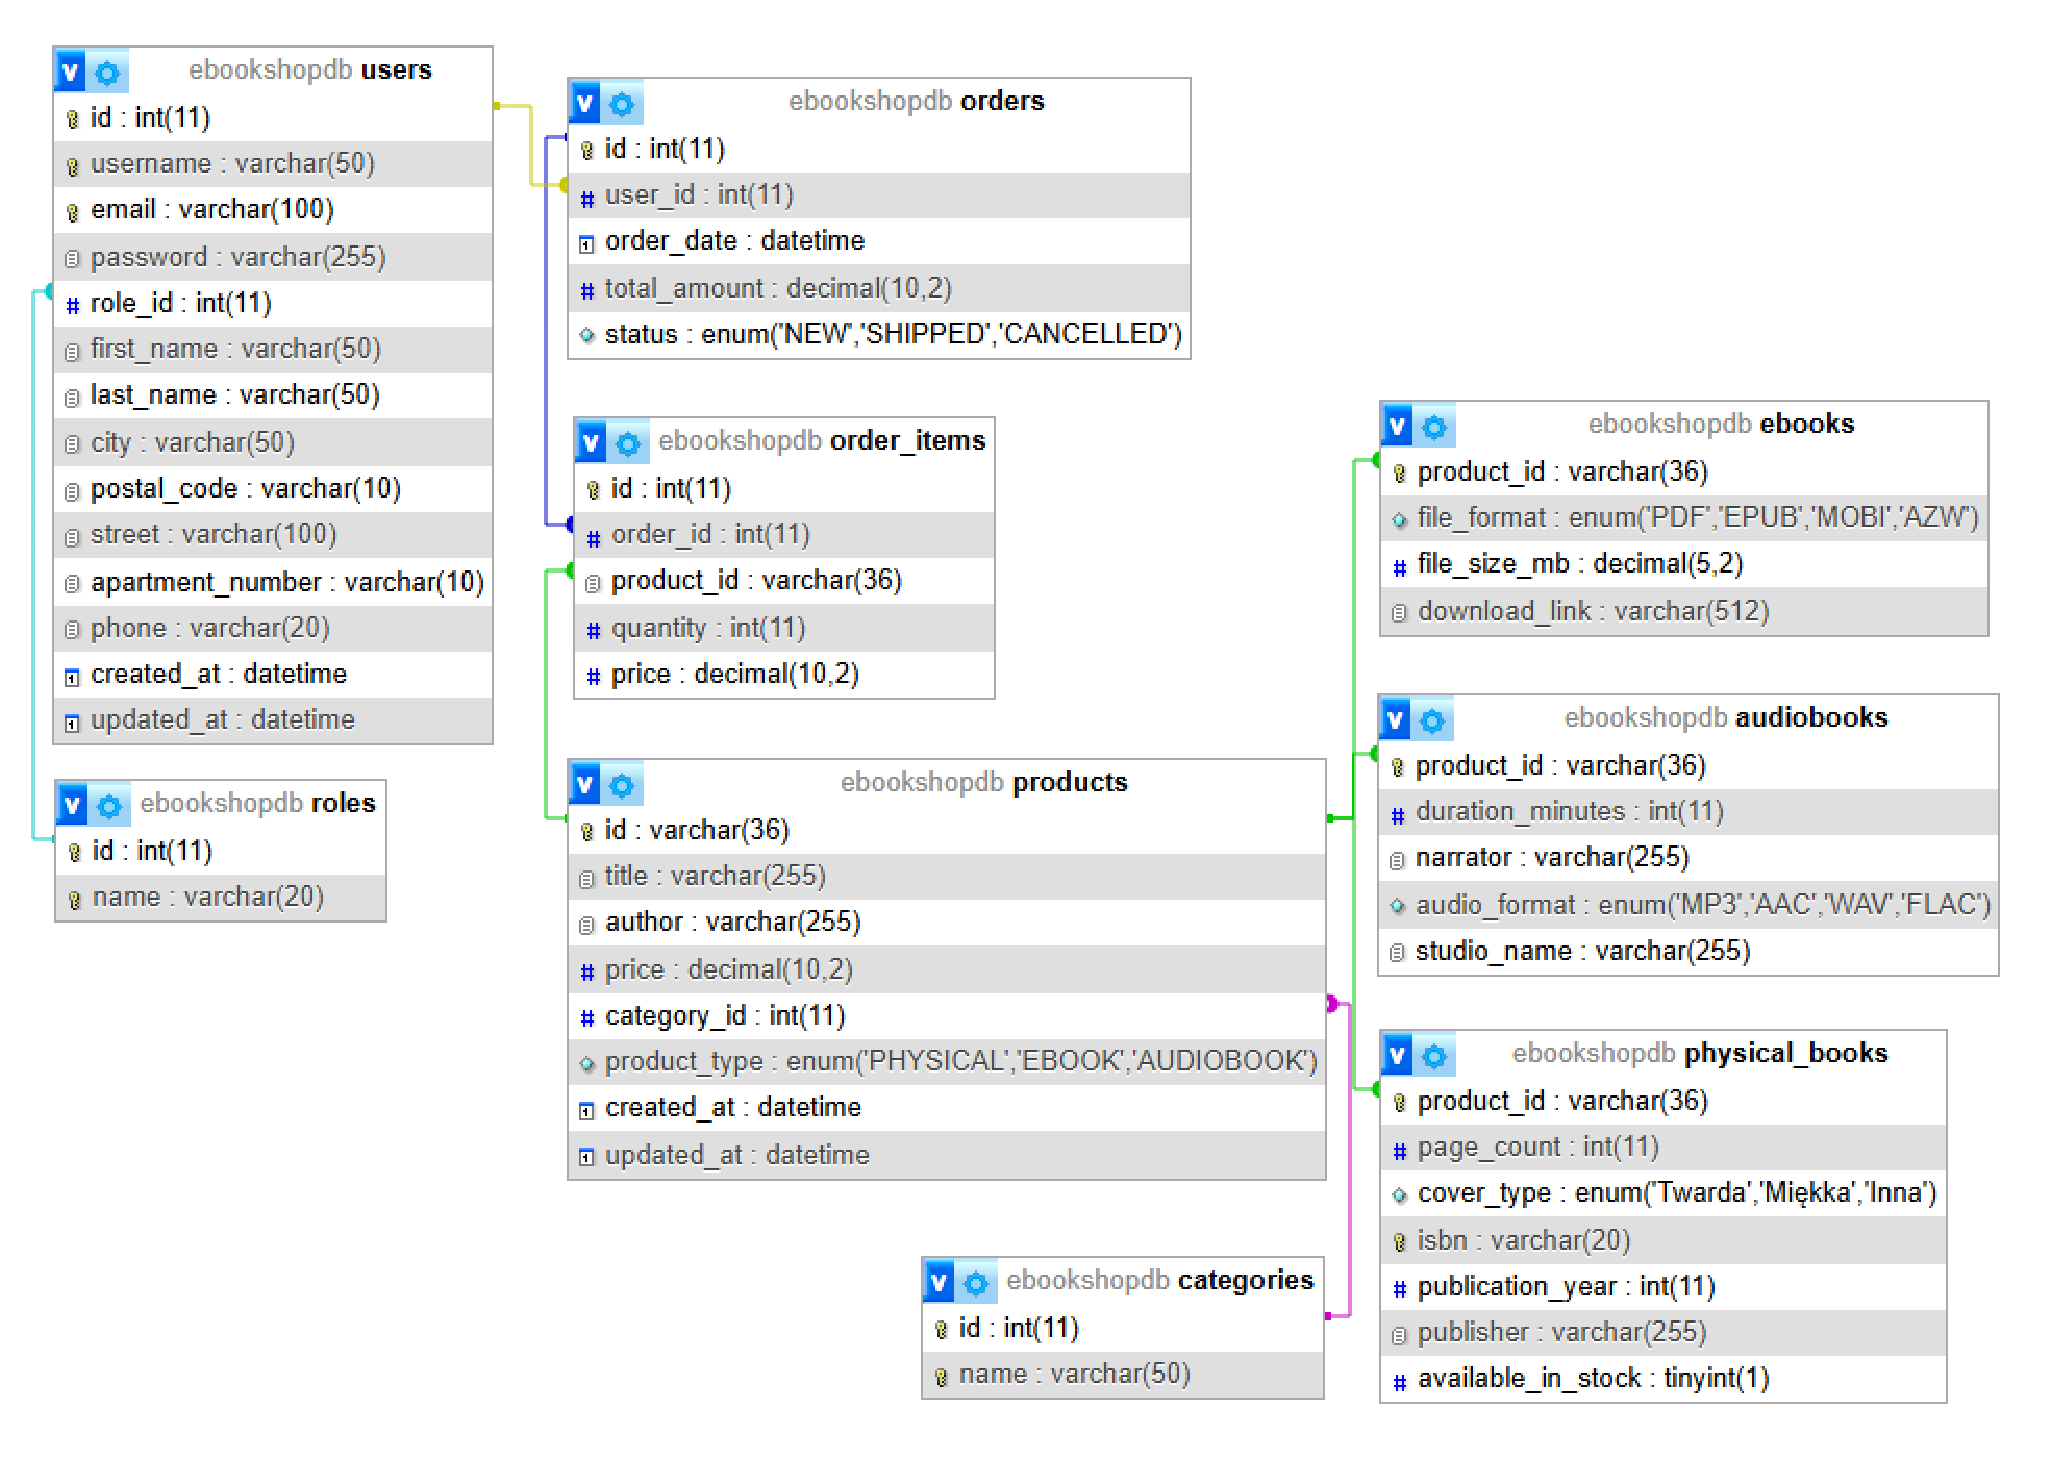
\includegraphics[width=\linewidth]{figures/fig_0004.eps}\\
    \caption{Diagram ERD bazy danych.\label{fig4}}
\end{figure}

% ------------------------------------------------------------------------

\section{Graficzny interfejs użytkownika}

% ------------------------------------------------------------------------

\subsection{Struktura GUI}

Graficzny interfejs użytkownika został stworzony w taki sposób, aby był przejrzysty, prosty w obsłudze, a także estetyczny wizualnie.
Do tworzenia GUI wykorzystana została biblioteka SWING, a do samego projektowania, rozszerzenie \texttt{SWING UI DESIGNER}.

Wszystkie elementy interfejsu graficznego przechowywane są w pakiecie \texttt{GUI}, podzielone są one na okna dostępne dla klientów oraz gości, a także okna administratora, dostępne 
w zależności od tego na konto, z jaką rolą, zaloguje się użytkownik. Struktura GUI zaprezentowana została na diagramie na \figurename~\ref{fig5}. Diagram utworzony został przy użyciu \url{https://www.drawio.com/}.
\begin{figure}[H]
    \centering
    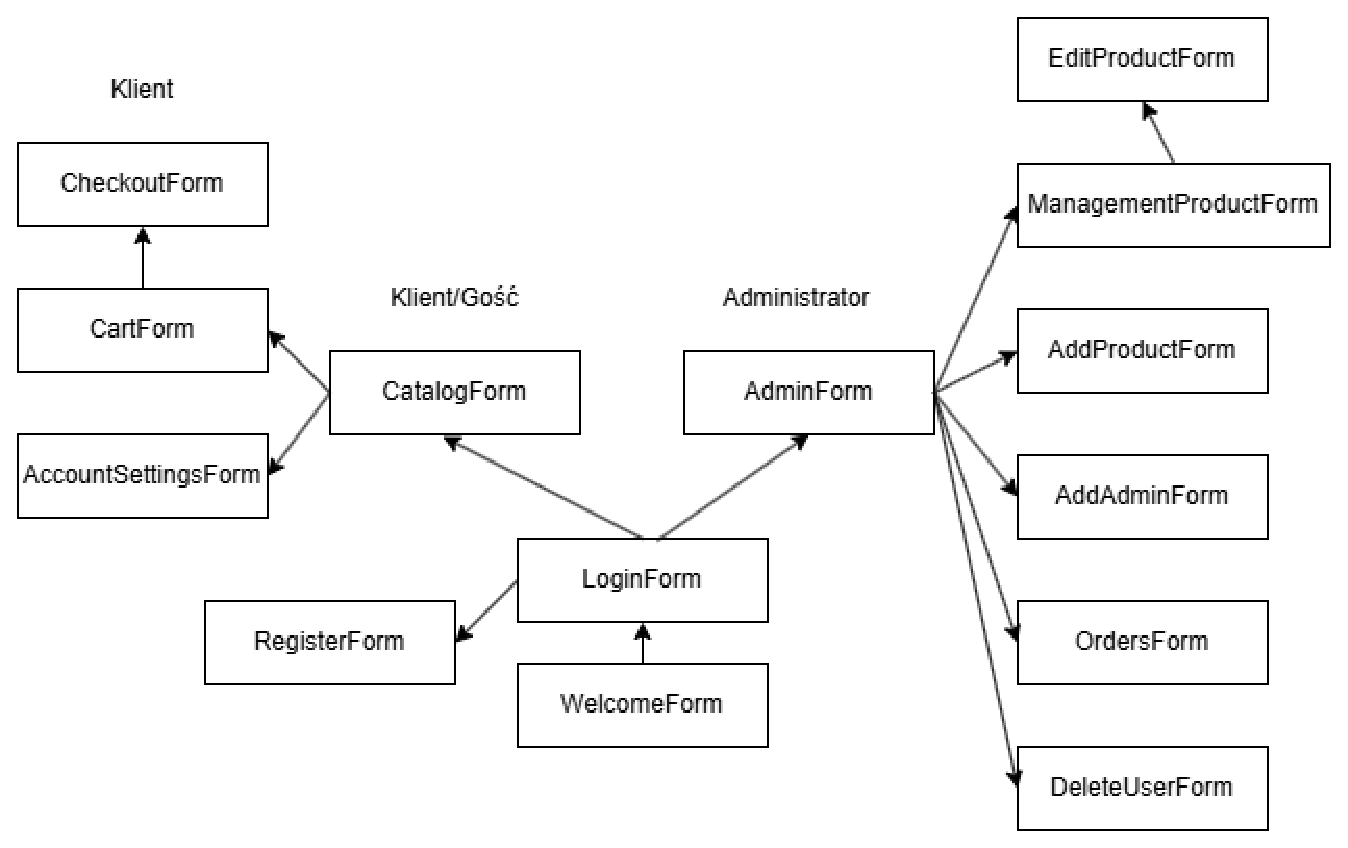
\includegraphics[width=\linewidth]{figures/fig_0005.eps}\\
    \caption{Diagram kolejnych okien aplikacji.\label{fig5}}
\end{figure}

% ------------------------------------------------------------------------

\subsection{Katalogi}

W sklepie internetowym często występują katalogi, takie jak np. katalog produktów i katalog zamówień. Jest to bardzo ważny element aplikacji, zatem konieczne jest aby były one czytelne oraz proste w korzystaniu z nich.

W projekcie wykorzystano metodę tworzenia katalogów, za pomocą dodawania do \texttt{JScrollPane} coraz to kolejnych paneli, zawierających dane na temat produktu (w przypadku katalogu produktów), a także przyciski funkcyjne
do np. dodawania przedmiotów do koszyka lub usuwania użytkowników (w przypadku panelu do usuwania użytkowników przez administratora). Wewnętrzną klasę paneli produktów prezentuje \listingname~\ref{panel}.
\lstinputlisting[caption= Klasa paneli z produktami, label=panel, style = javaStyle]{src/panel.java}

% ------------------------------------------------------------------------

\subsection{Sortowanie}

W tym przypadku katalogu produktów istotna jest również możliwość sortowania i filtorwania listy produktów. W tym celu wykorzystane zostały standardowe pakiety i klasy Javy takie jak np. \texttt{Collectors}.
Metoda \texttt{filterProducts} wykorzystuje strumień \texttt{stream} do filtrowania produktów na podstawie wybranego typu i kategorii, a następnie zbiera wyniki z powrotem do listy za pomocą \listingname~\ref{sort}.
Sortowanie natomiast odbywa się za pomocą metody \texttt{sort}, wywoływanej dla \texttt{mutableList}.\figurename~\ref{fig6} przedstawia implementację tych funkcjonalności.
\lstinputlisting[caption= Metody filtorwania oraz sortowania, label=sort, style = javaStyle]{src/sort.java}
\chapter{Harmonogram realizacji projektu}
\label{cha:harmonogram}

\section{Diagram Ganta pracy}

Na \figurename~\ref{fig6} przedstawiono diagram, zawierający informacje o kolejności podejmowanych działań oraz ich długości pracy.
Diagram utworzony został przy użyciu \url{https://www.drawio.com/}.
\begin{figure}[H]
    \centering
    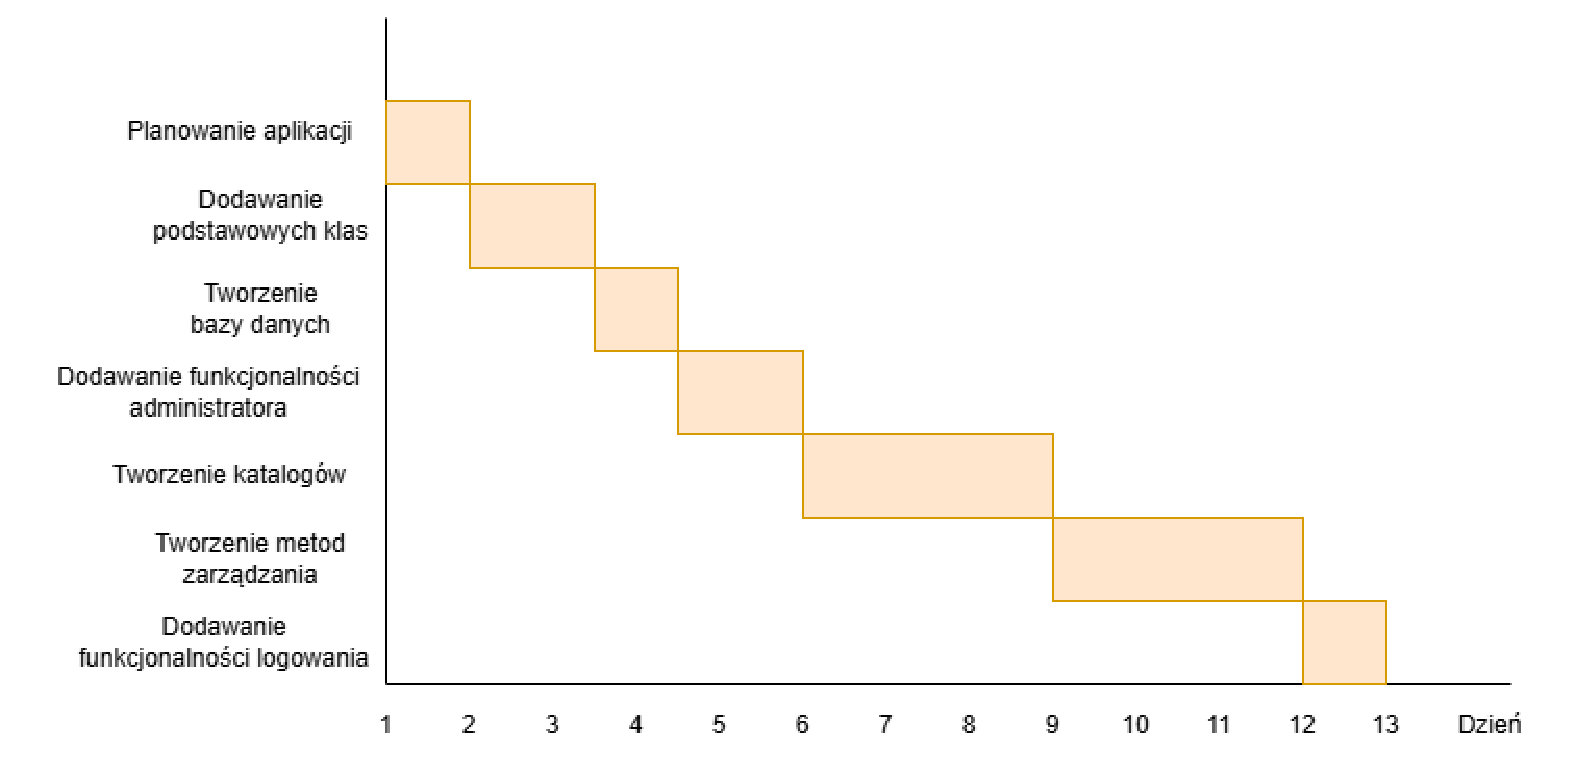
\includegraphics[width=\linewidth]{figures/fig_0006.eps}\\
    \caption{Diagram Ganta pracy.\label{fig6}}
\end{figure}

Praca nad projektem została rozpoczęta 31 maja, a zakończyły się 12 czerwca, trwały one 13 dni, po 5 godzin dziennie, a etapy pracy zostały rozłożone tak, aby nie nakładały się na siebie i pozwalały na skupienie się na dodawaniu konktretnych funkcjonalności.

Najbardziej wymagającą i czasochłonną częścią prac okazuje się być zrealizowanie funkcjonalnych, przystępnych i estetycznych wizualnie 
katalogów produktów, zamówień i użytkowników.

\section{Repozytorium i system kontroli wersji}
Całość projektu wraz z wyeksportowaną bazą danych zostały przeniesione do repozytorium GitHub \url{https://github.com/Buczul/Symulator_sklepu_internetowego_repo}.
\chapter{Prezentacja warstwy użytkowej projektu}
\label{cha:wartstwa uzytkowa}

\section{Logowanie}

Po uruchomieniu aplikacji pojawia się okno ładowania, które szybko znika, a otwarty zostaje panel logowania, przedstawiony na \figurename~\ref{fig10}. Dostępne jest tutaj logowanie na konto, rejestracja nowego użytkownika,
a także logowanie jako gość, należy jednak pamiętać że gość ma jedynie dostęp do przeglądania oferty.
\begin{figure}[H]
    \centering
    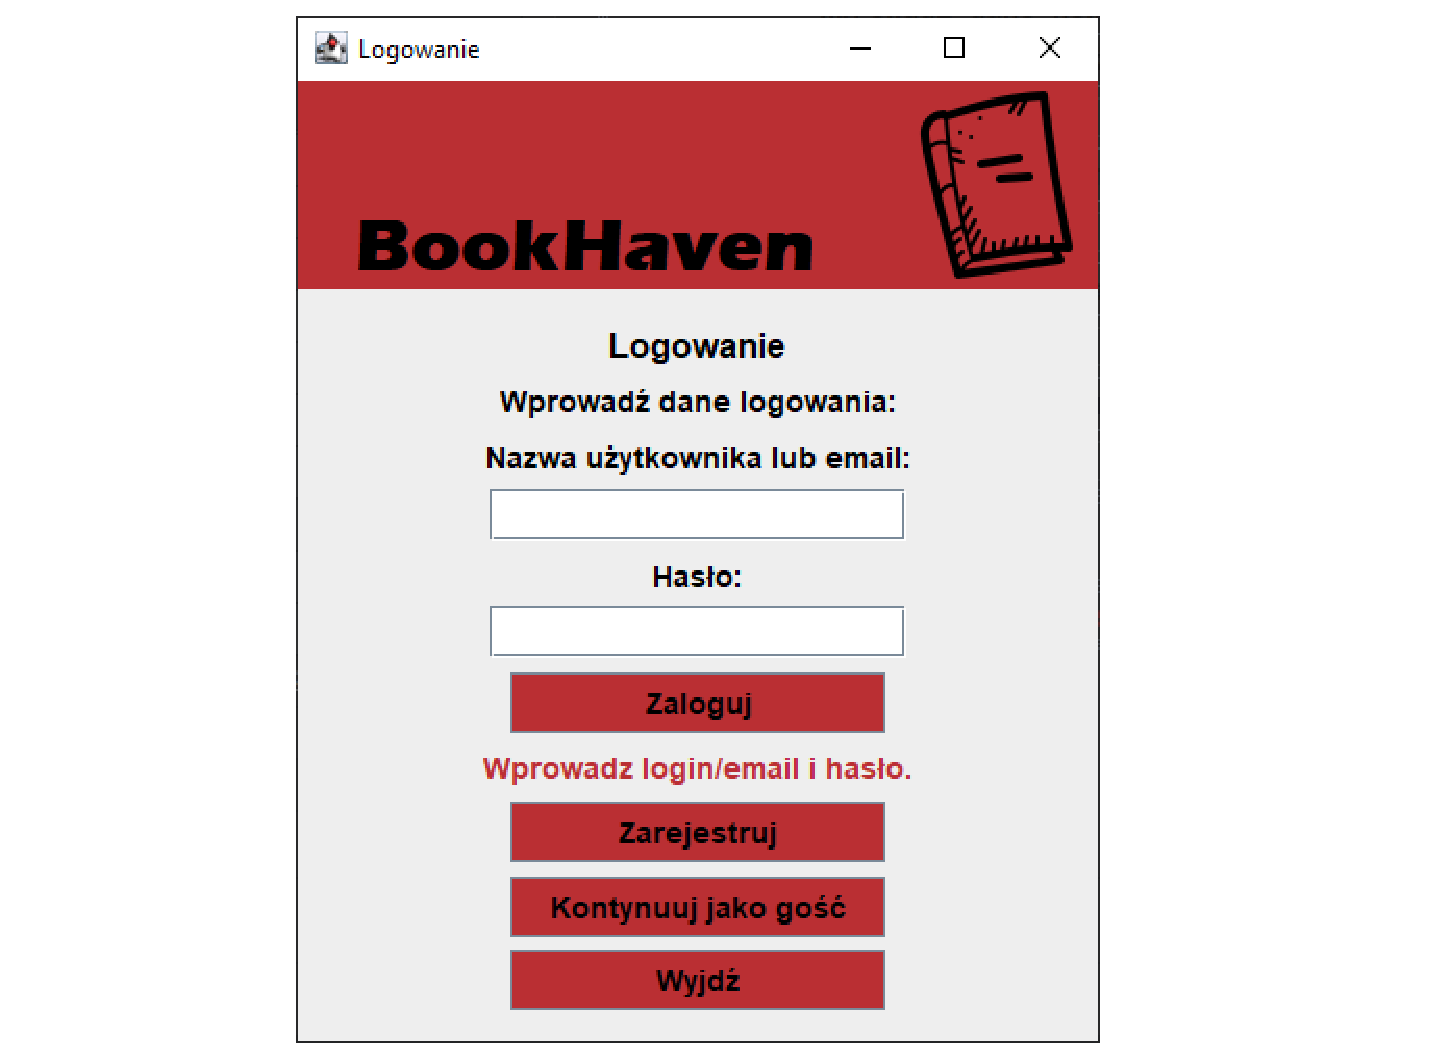
\includegraphics[width=\linewidth]{figures/fig_0010.eps}\\
    \caption{Panel logowania.\label{fig10}}
\end{figure}

\section{Panel klineta i gościa}

Po zalogowaniu na konto użytkownika otworzy się okno z sortowalnym i filtrowalnym katalogiem produktów dostpęnych w aplikacji. Zostało to przedstawione
na \figurename~\ref{fig12}. Dostępne są tutaj opcje zmiany ustawień konta (zmiana danych do późniejszej wysyłki), dodawanie produktów do koszyka, a także
wejście do koszyka, wraz z możliwością złożenia zamówienia przez klienta.
\begin{figure}[H]
    \centering
    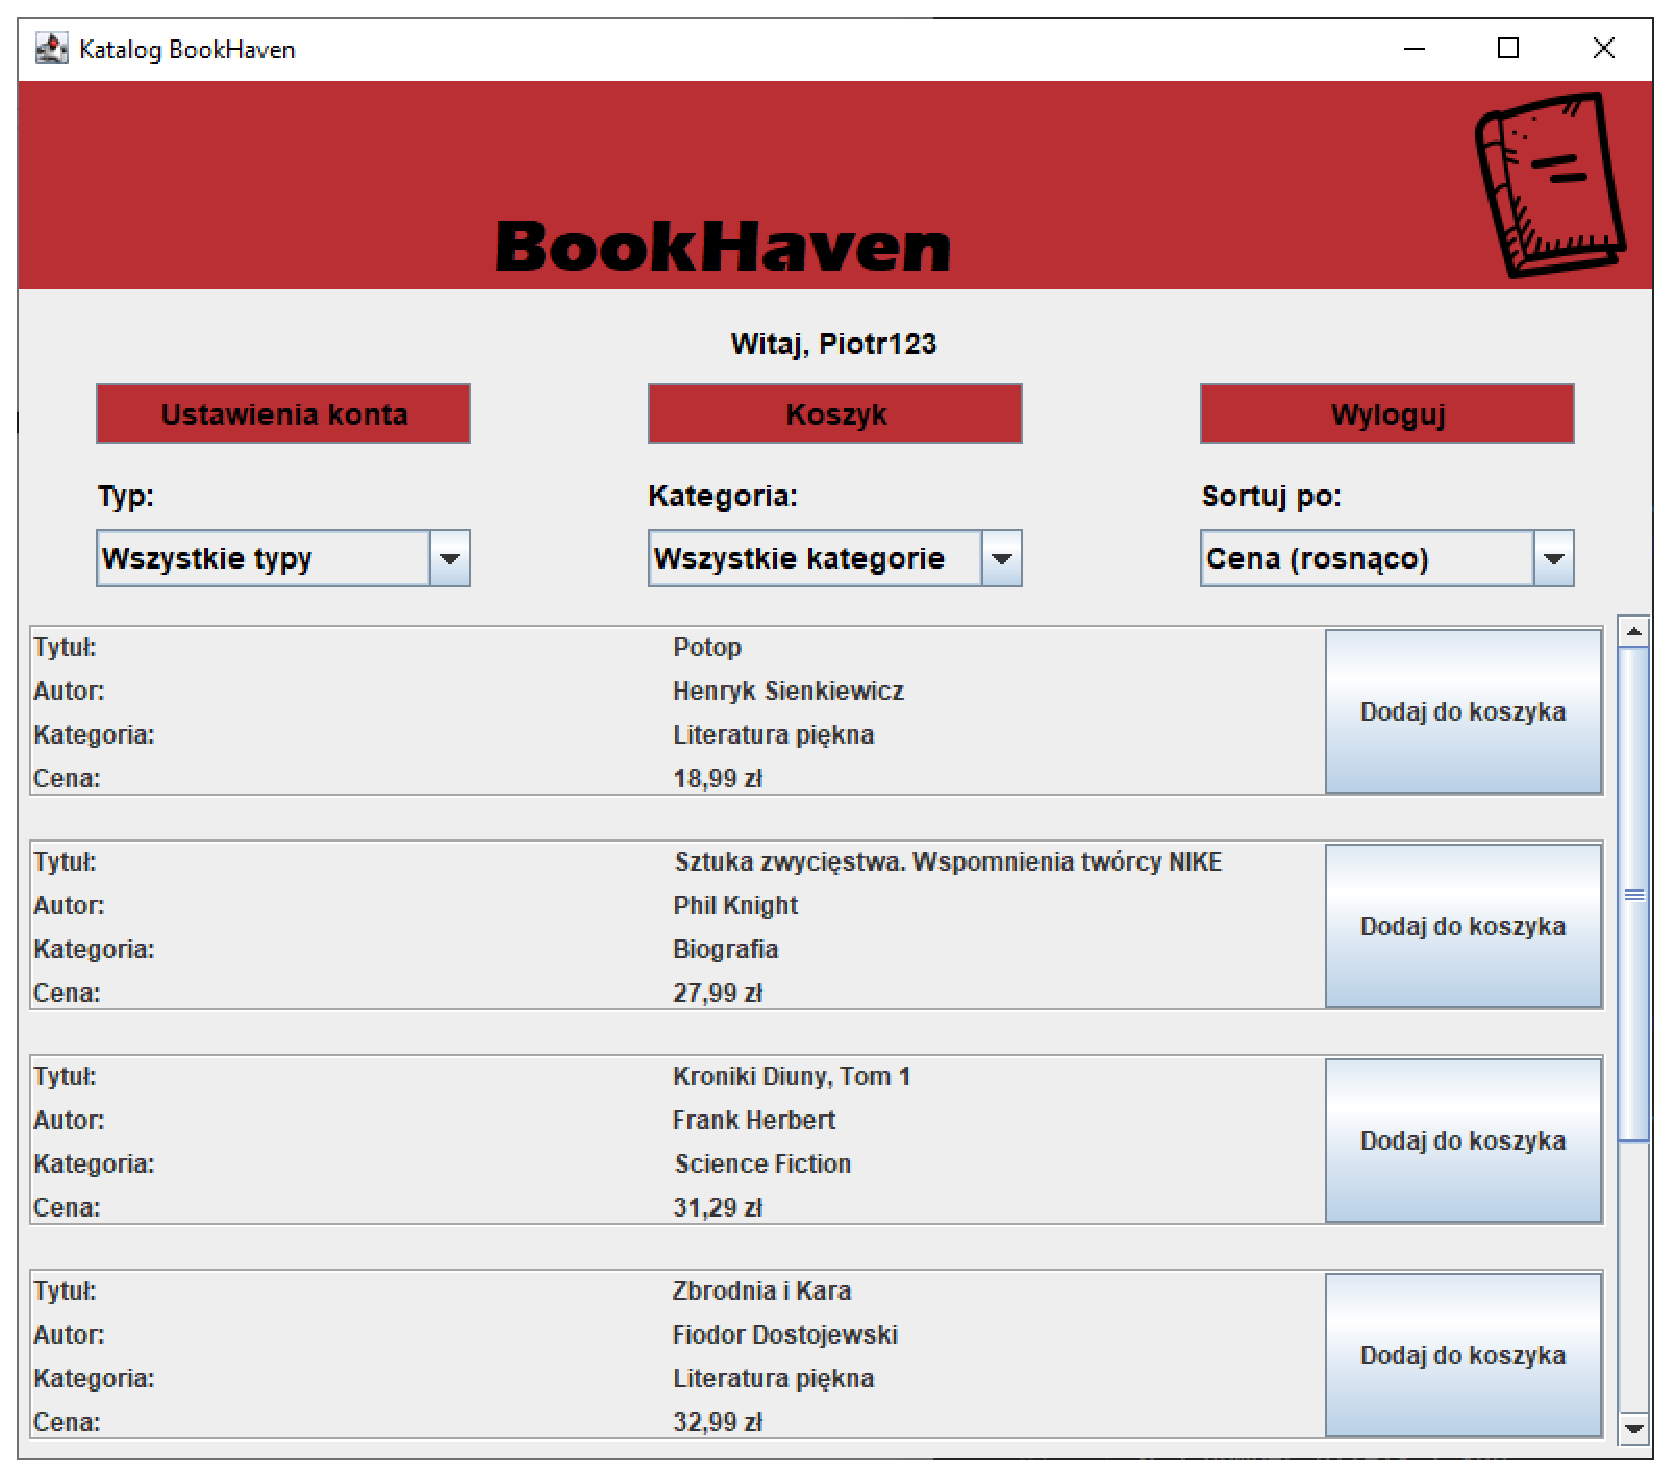
\includegraphics[width=\linewidth]{figures/fig_0012.eps}\\
    \caption{Panel klienta i gościa.\label{fig12}}
\end{figure}

\section{Panel administratora}

Po zalogowaniu na konto administratora (konto testowe o nazwie użytkownika "admin" oraz haśle "admin"), wyświetlony zostaje panel z możliwymi do podjęcia, przez niego, działaniami.
Panel ten przedstawiony jest na \figurename~\ref{fig11}. Administrator ma możliwość usuwania użytkowników z bazy, dodawania nowych administratorów oraz nowych produktów do bazy.
Zarządzanie produktami daje administratorowi narzędzia do usuwania i edycji istniejących produktów. Administrator może również zarządzać zamówieniami (przeglądać wszystkie zamówienia oraz zmieniać ich status).


\begin{figure}[H]
    \centering
    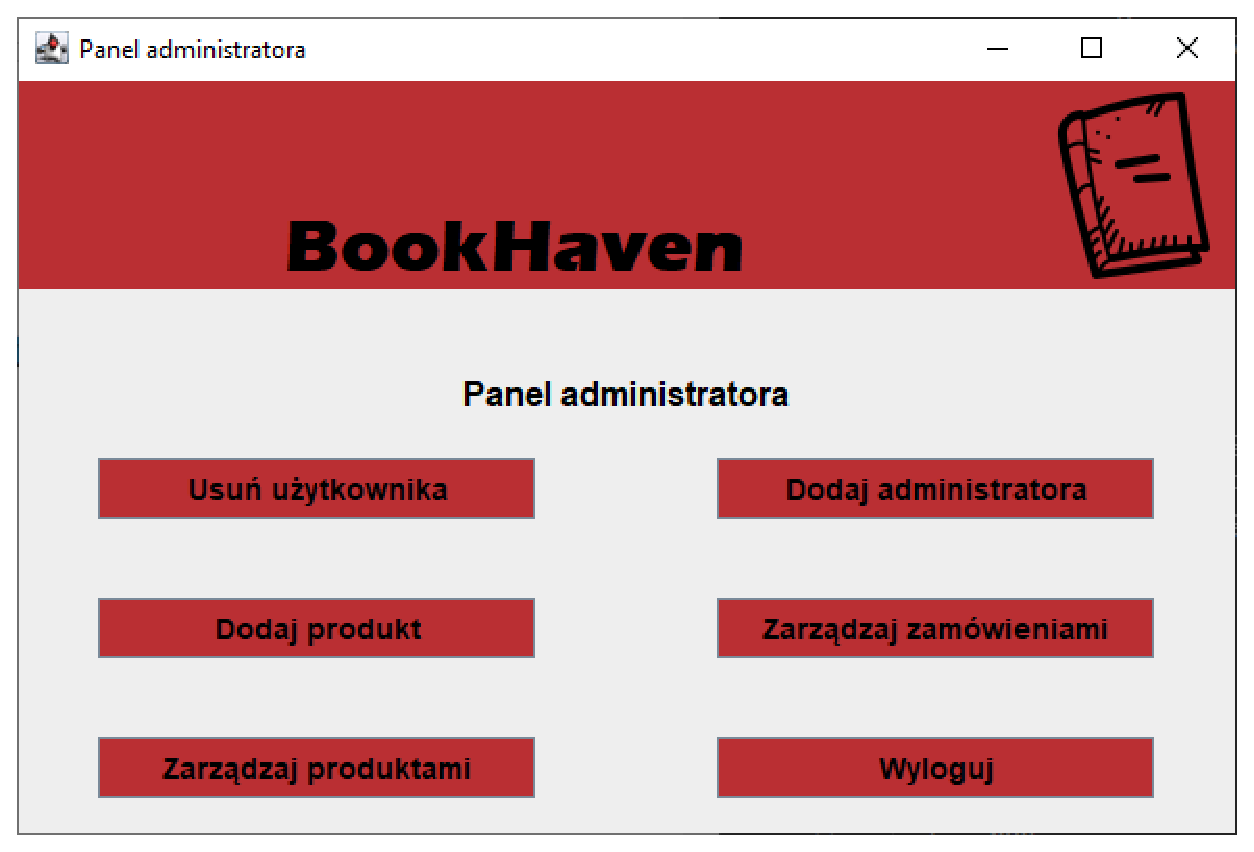
\includegraphics[width=\linewidth]{figures/fig_0011.eps}\\
    \caption{Panel administratora.\label{fig11}}
\end{figure}
\chapter{Podsumowanie}
\label{cha:podsumowanie}

Projekt "Symulator sklepu internetowego" został zrealizowany zgodnie z założeniami i wymaganiami 
określonymi na początku prac. Aplikacja umożliwia użytkownikom pełne korzystanie z funkcjonalności sklepu internetowego, w tym rejestrację, logowanie, przeglądanie oferty, dodawanie produktów do koszyka oraz składanie zamówień. Administratorzy mają możliwość zarządzania użytkownikami, produktami i zamówieniami, co zapewnia kompleksową obsługę systemu.

Interfejs graficzny został zaprojektowany w sposób przejrzysty i intuicyjny, co ułatwia nawigację zarówno klientom, jak i administratorom. Wykorzystanie bazy danych MySQL pozwoliło na efektywne przechowywanie i zarządzanie danymi, a zastosowanie podejścia obiektowego Javy oraz korzystanie z biblioteki SWING zapewniło wysoką wydajność i skalowalność aplikacji.

Projekt spełnił wszystkie założone cele, a także uwzględnił wymagania niefunkcjonalne, takie jak szybkość działania, niezawodność i estetyka interfejsu. Dalszy rozwój aplikacji może obejmować rozszerzenie funkcjonalności, np. dodanie nowych metod płatności czy tworzenie nowych kategorii produktów.

Podsumowując, projekt stanowi kompleksowe rozwiązanie symulujące działanie sklepu internetowego, które może służyć jako podstawa do dalszych prac rozwojowych.

% Wyłączenie działania ulem na czas bibliografii
\renewcommand{\emph}[1]{\textit{#1}}
% Bibliografia
% Dodanie bibliografi do spisu treści


% Przywrócenie działania ulem
\renewcommand{\emph}[1]{\uline{#1}}

\clearpage
% Dodanie spisu rysunków do spisu treści
\addcontentsline{toc}{section}{\textbf{Spis rysunków}}
\listoffigures
\clearpage

% Dodanie spisu tabel do spisu treści
\addcontentsline{toc}{section}{\textbf{Spis tabel}}
\listoftables
\clearpage


\clearpage

% Dodanie spisu listingow do spisu treści
\addcontentsline{toc}{section}{\textbf{Spis listingów}}
\lstlistoflistings
\clearpage
\clearpage

% \appendix

\appendix
\chapter{Oświadczenie studenta o samodzielności pracy}
\label{appendix:A}

\begin{figure}[H]
  \centering
  \includegraphics[width=\linewidth]{figures/statementB.eps}
\end{figure}



\end{document}